
Here's the adapted section discussing Fuzzy C-Means instead of K-Means, preserving the original structure and style but adjusted for the fuzzy clustering approach:



\subsection*{\subsection{Fuzzy C-Means}}

We have tested on each dataset 57 different configurations of the Fuzzy C-Means (FCM) algorithm, by using the fuzziness parameter m (with values from 1.5 to 4.0) and varying the number of clusters (n\_clusters) between 2 and 20. For each configuration, we ran the algorithm 10 times to mitigate the effects of initialization randomness. This resulted in a total of 570 runs of the FCM algorithm per dataset. From the evaluation metrics extracted in these runs, we analyze the impact of the key hyperparameters and derive insights through statistical analysis.


\subsection*{\subsubsection{Preliminary Study}}

We first explored preliminary patterns in the measured metrics and the influence of hyperparameters on clustering performance.


Figure \ref{fig:metrics_corr} illustrates the relationships between the various metrics for the FCM algorithm. This matrix plot highlights the correlations between metrics (lower triangle), histogram distributions (diagonal), and scatterplots of metric values (upper triangle). A notable observation is the interaction between the fuzziness parameter and metrics like Silhouette and DBI. For instance, while lower fuzziness (mm) often improves silhouette scores due to sharper cluster boundaries, it can lead to higher DBI values, which might indicate a trade-off between cluster compactness and interpretability. Similar trends are observed across all datasets, though the degree of correlation varies.


\begin{figure}[h]
\centering
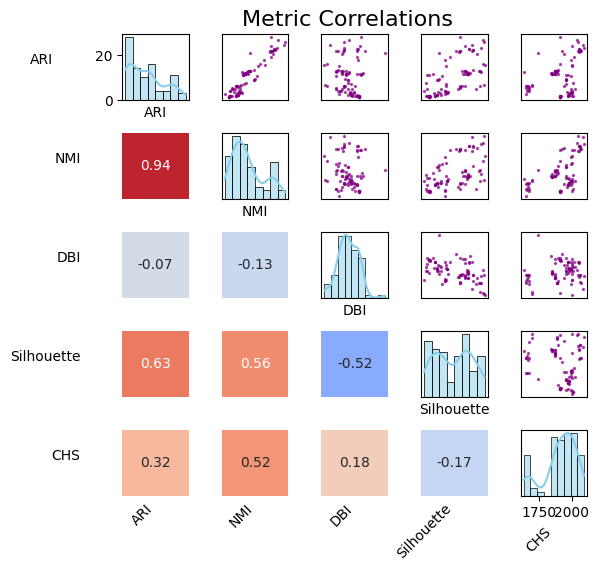
\includegraphics[width=0.7\textwidth]{figures/FuzzyCMeans/metrics_correlations_matrix.png}
\caption{Metrics correlations summary for Fuzzy C-Means}
\label{fig:metrics_corr}
\end{figure}


Additionally, Figure \ref{fig:pairplot} shows hyperparameter pairwise relationships, particularly the impact of fuzziness (mm) and number of clusters (n_clustersn\_clusters) on clustering quality and execution time. Across datasets, higher fuzziness values consistently resulted in more computationally expensive runs, likely due to the increased complexity of assigning membership values. Interestingly, for datasets like Pen-based (10 classes), intermediate cluster counts (e.g., n_clusters=10n\_clusters = 10) aligned closely with ground truth and yielded better metrics, such as ARI and NMI. Conversely, for Mushroom (2 classes), smaller values of n_clustersn\_clusters and lower fuzziness performed better.


\begin{figure}[H]
\centering
\begin{subfigure}{0.49\textwidth}
\centering
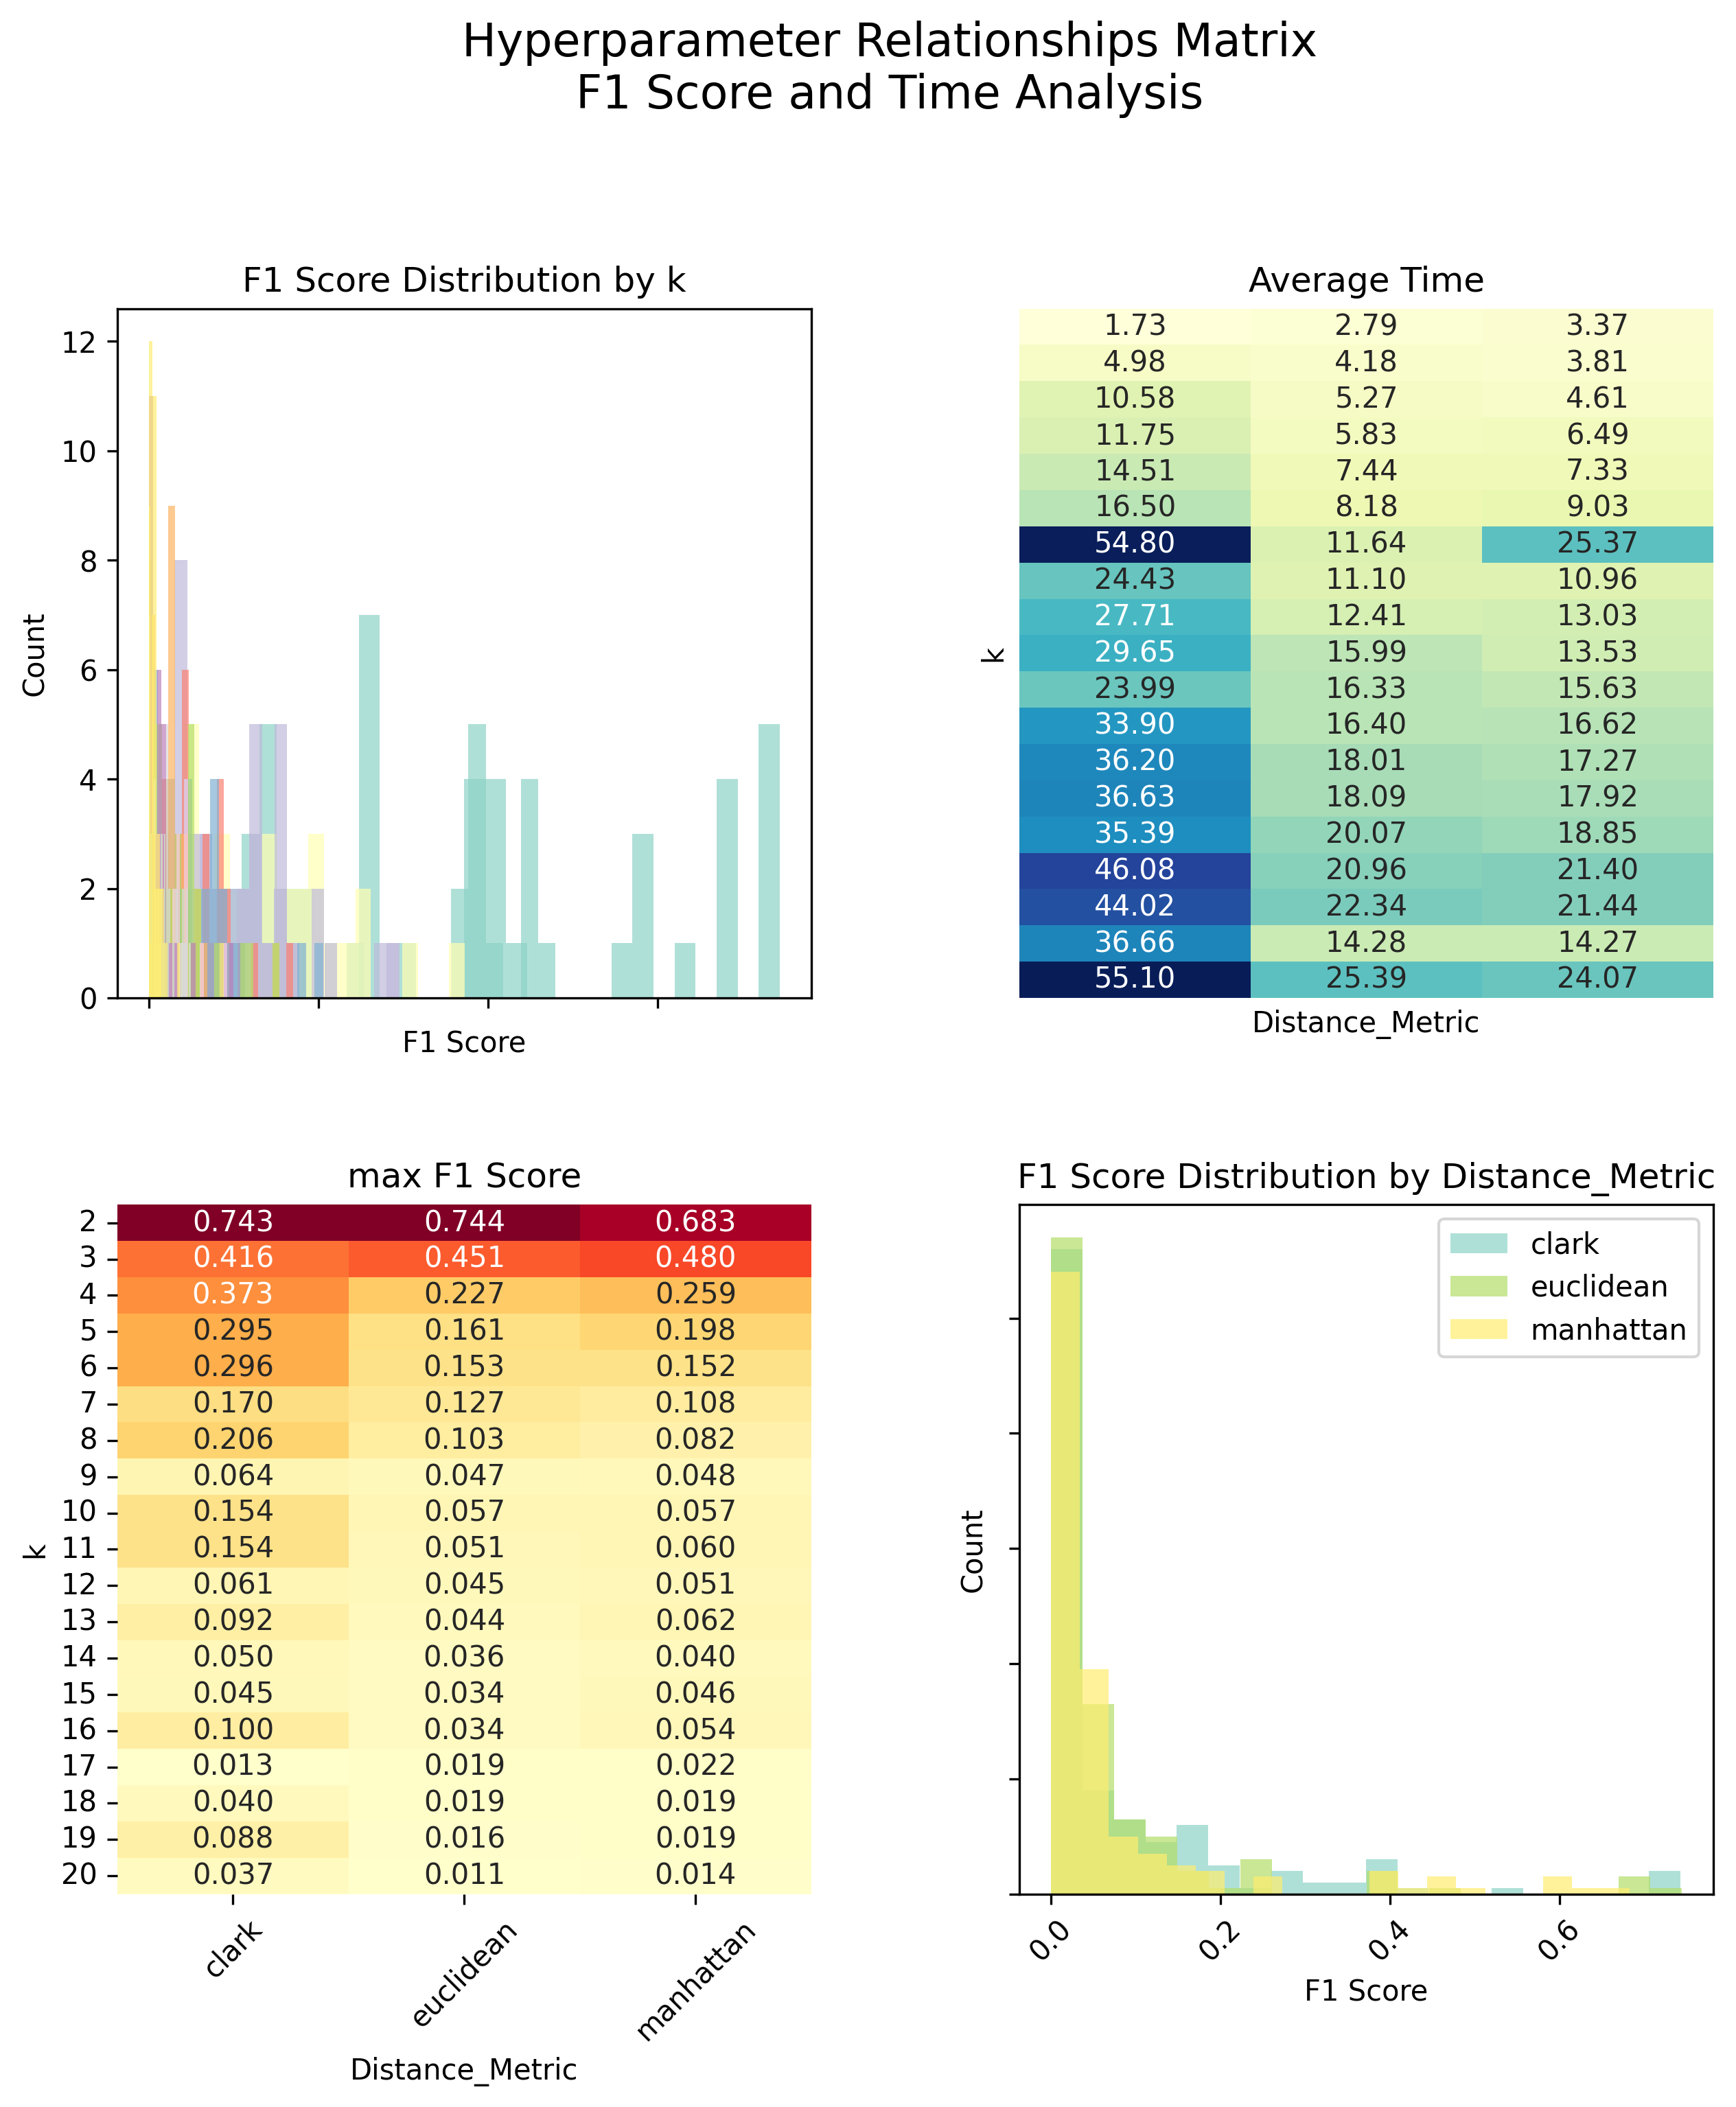
\includegraphics[width=\linewidth]{figures/mushroom_hyperparameter_pairplot_matrix.png}
\caption{Mushroom pairplot matrix for FCM}
\end{subfigure}
\hfill
\begin{subfigure}{0.49\textwidth}
\centering
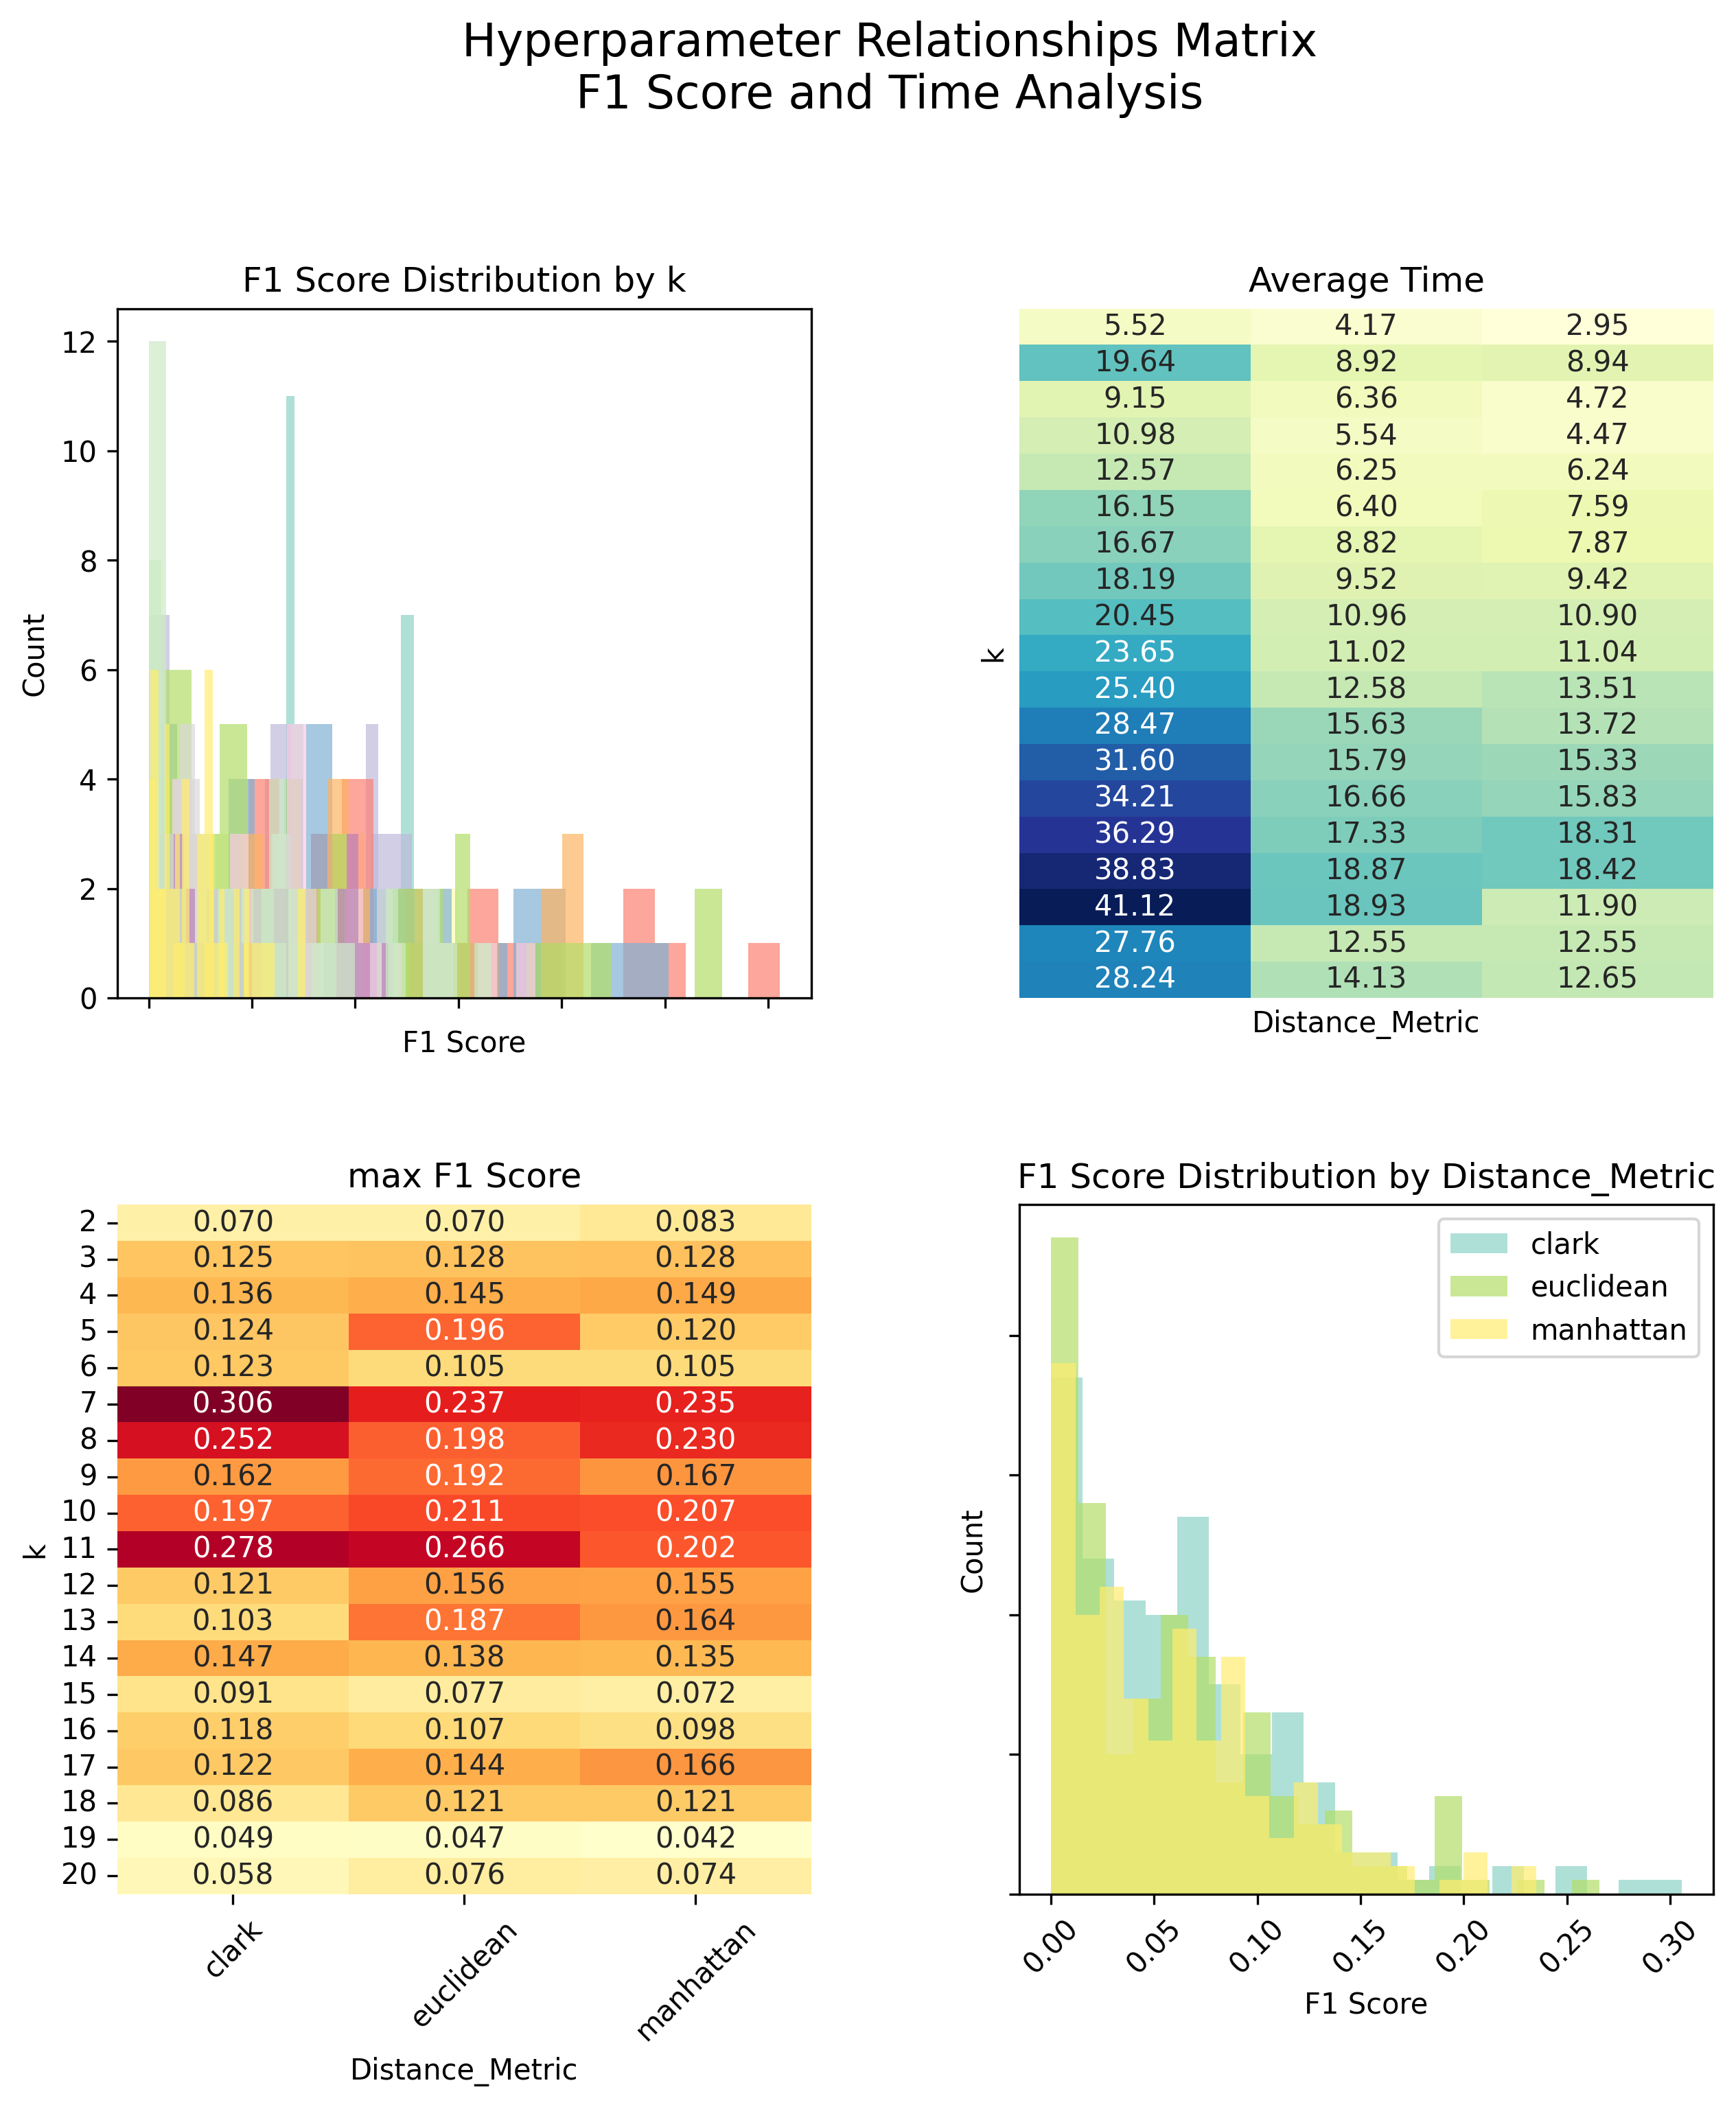
\includegraphics[width=\linewidth]{figures/penbased_hyperparameter_pairplot_matrix.png}
\caption{Pen-based pairplot matrix for FCM}
\end{subfigure}
\caption{Hyperparameter pairplot matrices based on clustering metrics and execution time for FCM}
\label{fig:pairplot}
\end{figure}


\subsection*{\subsubsection{Statistical Analysis}}

For the statistical analysis, we used Friedman tests to assess whether significant differences exist among metrics for varying values of fuzziness and number of clusters. With a confidence level of α=0.15\alpha = 0.15, the results consistently indicate significant differences across all datasets when varying both hyperparameters.


\textit{Note:} Due to the large volume of results, only the most relevant findings are discussed here. The full set of results can be accessed in the \texttt{code} folder under \texttt{Analysis/plot_and_tables/FuzzyCMeansReports}.


\subsubsection*{Fuzziness Parameter (mm):}

Post-hoc Nemenyi tests revealed that lower values of mm (e.g., 1.5) typically resulted in sharper cluster assignments, reflected in higher ARI and NMI values. However, excessive sharpness (e.g., m=1.5m = 1.5) can negatively impact interpretability and increase DBI values. Intermediate fuzziness values (e.g., m=2.0m = 2.0) often strike a balance between cluster quality and computational efficiency. These findings were consistent across all datasets.


\subsubsection*{Number of Clusters (n_clustersn\_clusters):}

\begin{enumerate}

\item Hepatitis: Lower cluster counts (e.g., n_clusters=2n\_clusters = 2) showed better ARI and Silhouette scores, aligning with the dataset's two-class structure.

\item Mushroom: Metrics like CHS favored smaller cluster counts, with n_clusters∈[2,4]n\_clusters \in [2, 4] achieving the best results. Silhouette scores corroborated these findings.

\item Pen-based: Higher cluster counts (n_clusters=10n\_clusters = 10) aligned with the dataset's class structure and yielded optimal ARI and NMI. Lower counts led to poor clustering quality, while overly high values showed diminishing returns.

\end{enumerate}

These findings confirm the sensitivity of FCM to both hyperparameters and its suitability for datasets with well-defined class structures.



\subsection*{Highlights from Tables}

\begin{itemize}

\item Pen-based Dataset: Optimal ARI (0.6242) and NMI (0.7073) achieved with n_clusters=10n\_clusters = 10 and m=2.0m = 2.0, reflecting its 10-class nature.

\item Mushroom Dataset: CHS (1962.91) supports n_clusters=6n\_clusters = 6 and m=1.5m = 1.5, showcasing the importance of small cluster counts in this two-class dataset.

\item Hepatitis Dataset: Lower n_clustersn\_clusters and fuzziness values provide better interpretability, with the highest ARI (0.1389) for m=1.5m = 1.5.

\end{itemize}

This adaptation integrates Fuzzy C-Means characteristics while maintaining your original narrative structure.

